% Created 2019-08-26 Mon 17:34
% Intended LaTeX compiler: lualatex
\documentclass[11pt]{article}
\usepackage{polyglossia}
\usepackage{graphicx}
\usepackage{grffile}
\usepackage{longtable}
\usepackage{wrapfig}
\usepackage{rotating}
\usepackage[normalem]{ulem}
\usepackage{amsmath}
\usepackage{textcomp}
\usepackage{amssymb}
\usepackage{capt-of}
\usepackage{hyperref}
\author{Vladimir Nikishkin}
\date{\today}
\title{}
\hypersetup{
 pdfauthor={Vladimir Nikishkin},
 pdftitle={},
 pdfkeywords={},
 pdfsubject={},
 pdfcreator={Emacs 26.2 (Org mode 9.1.9)}, 
 pdflang={English}}
\begin{document}

\tableofcontents



\section{noweb}
\label{sec:org44d37e9}
\section{SICP [14/362]}
\label{sec:org4c30d44}
\begin{verbatim}
header-args: :noweb yes
\end{verbatim}

\begin{enumerate}
\item {\bfseries\sffamily TODO} Chapter 1: Building abstractions with procedures [14/47]
\label{sec:orgf001285}
\begin{enumerate}
\item Snippet
\label{sec:org8bbb6b9}
\lstset{language=Lisp,label= ,caption= ,captionpos=b,numbers=none}
\begin{lstlisting}
(* (+ 2 (* 4 6))
   (+ 3 5 7))
\end{lstlisting}

\item Thought
\label{sec:orgda4fa63}
Tree accumulation is the process of computing a thing by traversing a tree.

\item {\bfseries\sffamily DONE} Figure 1.1
\label{sec:org2768e20}
\noindent\textbf{CLOSED:} \textit{[2019-08-20 Tue 14:35]}\\
For the sake of pedagogical clarity, I have formatted it as a picture.
\begin{center}
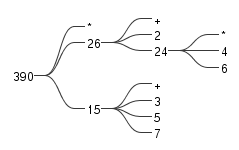
\includegraphics[width=.9\linewidth]{figure-1-1-mm.png}
\end{center}
;

\begin{center}
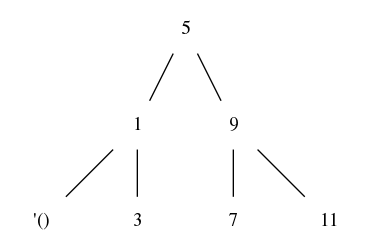
\includegraphics[width=.9\linewidth]{figure-1-1-dot.png}
\end{center}

\item Snippet
\label{sec:orgc6ce1a5}
\#+name square
\lstset{language=Lisp,label= ,caption= ,captionpos=b,numbers=none}
\begin{lstlisting}
(define (square x) (* x x))
(define (sum-of-squares x y)
  (+ (square x) (square y)))
(sum-of-squares 3 4)
\end{lstlisting}

\item {\bfseries\sffamily DONE} Exercise 1.1
\label{sec:orgba9b1e5}
\noindent\textbf{CLOSED:} \textit{[2019-08-20 Tue 14:23]}\\
\lstset{language=Lisp,label= ,caption= ,captionpos=b,numbers=none}
\begin{lstlisting}
(define (disp sexp)
  (display sexp)
  (newline))
(disp 10)
(disp (+ 2 3 4))
(disp (- 9 1))
(disp (/ 6 2))
(disp (+ (* 2 4) (- 4 6)))
(define a 3)
(define b (+ a 1))
(disp (+ a b (* a b)))
(disp (= a b))
(disp
 (if (and (> b a) (< b (* a b )))
     b
     a))
(disp (cond ((= a 4) 6)
     ((= b 4) (+ 6 7 a))
     (else 25)))
(disp (+ 2 (if (< b a) b a)))
(disp (* (cond ((> a b) a)
            ((< a b) b)
            (else -1)) 
         (+ a 1)))
\end{lstlisting}

\item {\bfseries\sffamily DONE} Exercise 1.2
\label{sec:orgaaf06aa}
\noindent\textbf{CLOSED:} \textit{[2019-08-20 Tue 14:25]}\\
\lstset{language=Lisp,label= ,caption= ,captionpos=b,numbers=none}
\begin{lstlisting}
(/ (+ 5 4 (- 2 (- 3 (+ 6 (/ 4 5))))) (* 3 (- 6 2) (- 2 7)))
\end{lstlisting}

\item {\bfseries\sffamily DONE} Exercise 1.3
\label{sec:orga2f8494}
\noindent\textbf{CLOSED:} \textit{[2019-08-20 Tue 14:35]}\\
\lstset{language=Lisp,label= ,caption= ,captionpos=b,numbers=none}
\begin{lstlisting}
(define (sum-of-squares x y)
  (+ (square x) (square y)))
(import (srfi 95))
(define (sum-of-two-max a b c)
  (let ((num_list (sort (list a b c) (lambda (a b) (if (> a b) a b)))))
   (sum-of-squares (car num_list) (cadr num_list))))
(sum-of-two-max 1 2 3)
\end{lstlisting}

\item {\bfseries\sffamily DONE} Exercise 1.4
\label{sec:org417bff1}
\noindent\textbf{CLOSED:} \textit{[2019-08-20 Tue 14:39]}\\
\lstset{language=Lisp,label= ,caption= ,captionpos=b,numbers=none}
\begin{lstlisting}
(define (a-plus-abs-b a b)
  ((if (> b 0) + -) a b))
(disp (a-plus-abs-b  3 4))
(disp (a-plus-abs-b  3 -4))
\end{lstlisting}

\item {\bfseries\sffamily DONE} Exercise 1.5
\label{sec:orge21ba0a}
\noindent\textbf{CLOSED:} \textit{[2019-08-20 Tue 14:50]}\\
\lstset{language=Lisp,label= ,caption= ,captionpos=b,numbers=none}
\begin{lstlisting}
(define (p) (p))
(define (test x y)
  (if (= x 0) 0 y))
(test 0 (p))
\end{lstlisting}

On my interpreter this code goes into an infinite recursion, which
makes sense, I guess, since the second argument to (test) is evaluated
before executing (test). However, if we only substitute \emph{p} into the
application of test and try to traverse the tree depth-first, this
code should be able to terminate successfully?

\item {\bfseries\sffamily DONE} Exercise 1.6
\label{sec:orgbde19b1}
\noindent\textbf{CLOSED:} \textit{[2019-08-21 Wed 14:05]}\\
The problem with this Alyssa's (new-if) is that both arguments would
be computed, so this (new-if) would be either very inefficient or even
not working at all in the case when one of the arguments is
infeasible.
Consider:

\lstset{language=Lisp,label= ,caption= ,captionpos=b,numbers=none}
\begin{lstlisting}
(import (chibi ast))
(import (chibi show))
 (define (disp sexp)
   (display sexp)
   (newline))
(define (new-if predicate then-clause else-clause)
  (cond (predicate then-clause)
        (else else-clause)))
(define a 1)
(define b 0)
(disp (if (not (= b 0)) (/ a b) a))
(new-if (not (= b 0)) (/ a b) a)
\end{lstlisting}

However, this issue can be solved using scheme macros.

\lstset{language=Lisp,label= ,caption= ,captionpos=b,numbers=none}
\begin{lstlisting}
(import (chibi ast))
(import (chibi show))
 (define (disp sexp)
   (display sexp)
   (newline))
(define-syntax new-if
  (syntax-rules ()
    ( (new-if predicate then-clause else-clause)
      (cond (predicate then-clause)
            (else else-clause))
    )
  )
)
(define a 1)
(define b 0)
(disp (if (not (= b 0)) (/ a b) a))
(disp (new-if (not (= b 0)) (/ a b) a))

\end{lstlisting}

The code above works as expected, because the macro does not evaluate
its arguments, and (cond) is a special form.

\item {\bfseries\sffamily DONE} Exercise 1.7
\label{sec:org35996d1}
\noindent\textbf{CLOSED:} \textit{[2019-08-22 Thu 12:52]}\\
This exercise is a very misleading one. On the first glance is seems
that this is just about formulating a good criterion. Make no mistake,
practically solving this task means really writing all this code
carefully.

The function we are interested in is:
\begin{equation}
\label{eq:5}
f(x) = \sqrt{x}
\end{equation}

The code given in the chapter before is equivalent to the following
Newton's method formula, where \(f_i\) denotes the next guess:
\begin{equation}
\label{eq:1} 
f_{i+1}_{} = \frac{f_i + \frac{x}{f_i}}{2}
\end{equation}

How on Earth does this formula even appear? Let's remember some
mathematics, namely, the Taylor series (variables unbound):
\begin{equation}
\label{eq:2}
 f(x) = f(x_{0}_{}) + f'(x_{0})(x-x_{0}) + o(x)
\end{equation}

Let us call `true' value of \(\sqrt{x}=f\). Let us call our first guess
\(f_{0}\). What is the value of the difference (error) between them?
Clearly, \(f-f_0\). Well, the problem is — we don't know \(f\). But we do
know \(f^2\). Therefore \(f^2-f^2_0\) is a number we know. What will be the
error on the next step of the algorithm? Let's find \(f_1\) as
\(f_1=f_0+\delta\). If \(\delta\) is not too big, we can use the Taylor
expansion from ref:eq:1 \(\delta\).
\begin{equation}
\label{eq:8}
E = f^2 - f_0^2 = f^2 - (f_0 + \delta)^2 \approx f^2 - f_0^2 - 2f_0\delta
\end{equation}


Be careful. What I expanded here is not the function value. It is the
\uline{error} value. Now, clearly we want our error to be as small as
possible, desirably as little as machine precision would allow. So
assuming \(E=0\), we get an equation to solve:
\begin{align}
\label{eq:9}
E=0 \leftrightarrow& f^2-f_0^2-2f_0\delta=0 \\
\delta =& \frac{f_0^2 -f^2 }{2f_0}
\end{align}

Remember though that we don't need just \(\delta\) here. We actually need
\(f_1\). But \(f_1\) is just \(f_0+\delta\).
\begin{align}
\label{eq:10}
f_1 = \frac{f^2 - f_0^2}{2f_0} + f_0
\end{align}
Now if you rearrange this formula, you will get exactly the formula
ref:eq:1.

The code below is copied from SICP verbatim and implements the
algorithm above.

\lstset{language=Lisp,label= ,caption= ,captionpos=b,numbers=none}
\begin{lstlisting}
(define (sqrt-iter guess x)
  (if (good-enough? guess x)
      guess
      (sqrt-iter (improve guess x) x)))
\end{lstlisting}

\lstset{language=Lisp,label= ,caption= ,captionpos=b,numbers=none}
\begin{lstlisting}
(define (improve guess x)
  (average guess (/ x guess)))
\end{lstlisting}

\lstset{language=Lisp,label= ,caption= ,captionpos=b,numbers=none}
\begin{lstlisting}
(define (good-enough? guess x)
  (< (abs (- (square guess) x)) 0.001))
(define (improve guess x)
  (average guess (/ x guess)))
(define (average x y)
  (/ (+ x y) 2))
(define (sqrt x)
  (sqrt-iter 1.0 x))

\end{lstlisting}

\#+name simple-newton
\lstset{language=Lisp,label= ,caption= ,captionpos=b,numbers=none}
\begin{lstlisting}
(import (chibi ast))
(import (chibi show))
 (define (disp sexp)
   (display sexp)
   (newline))

(define (sqrt-iter guess x)
  (if (good-enough? guess x)
      guess
      (sqrt-iter (improve guess x) x)))
(define (good-enough? guess x)
  (< (abs (- (square guess) x)) 0.001))
(define (improve guess x)
  (average guess (/ x guess)))
(define (average x y)
  (/ (+ x y) 2))
(define (sqrt x)
  (sqrt-iter 1.0 x))

(sqrt 9)
\end{lstlisting}

An example of how this fails on small numbers:

\lstset{language=Lisp,label= ,caption= ,captionpos=b,numbers=none}
\begin{lstlisting}

(square (sqrt 0.0004))
\end{lstlisting}

An example of why this fails on big numbers I didn't manage to
craft. Perhaps chibi-scheme has some clever way to deal with rounding?
Anyway — here is the code:
\lstset{language=Lisp,label= ,caption= ,captionpos=b,numbers=none}
\begin{lstlisting}

(square (sqrt 9999999999.0))
\end{lstlisting}

Why exactly this is not very good algorithms is a good question. The
derivative of the square is well-defined near the 0, although the
derivative of the square root is not. Therefore, the equation ref:eq:8
become very imprecise. As we see, big number seem to be working fine
in my scheme implementation.

Let us write a better sqrt-iter?.

\lstset{language=Lisp,label= ,caption= ,captionpos=b,numbers=none}
\begin{lstlisting}
(define (sqrt-iter guess x)
 (let ((better-guess (improve guess x)))
  (if (good-enough? guess (square better-guess))
      better-guess
      (sqrt-iter better-guess x))))
\end{lstlisting}

\lstset{language=Lisp,label= ,caption= ,captionpos=b,numbers=none}
\begin{lstlisting}
(import (chibi ast))
(import (chibi show))
 (define (disp sexp)
   (display sexp)
   (newline))

(define (sqrt-iter guess x)
 (let ((better-guess (improve guess x)))
  (if (good-enough? guess (square better-guess))
      better-guess
      (sqrt-iter better-guess x))))
(define (good-enough? guess x)
  (< (abs (- (square guess) x)) 0.001))
(define (improve guess x)
  (average guess (/ x guess)))
(define (average x y)
  (/ (+ x y) 2))
(define (sqrt x)
  (sqrt-iter 1.0 x))

\end{lstlisting}

\lstset{language=Lisp,label= ,caption= ,captionpos=b,numbers=none}
\begin{lstlisting}
(import (chibi ast))
(import (chibi show))
 (define (disp sexp)
   (display sexp)
   (newline))

(define (sqrt-iter guess x)
 (let ((better-guess (improve guess x)))
  (if (good-enough? guess (square better-guess))
      better-guess
      (sqrt-iter better-guess x))))
(define (good-enough? guess x)
  (< (abs (- (square guess) x)) 0.001))
(define (improve guess x)
  (average guess (/ x guess)))
(define (average x y)
  (/ (+ x y) 2))
(define (sqrt x)
  (sqrt-iter 1.0 x))

(square (sqrt 0.0004))
\end{lstlisting}

Works faster and gives a better result. Seemingly. QED\footnote{This exercise took me 7 hours.}.

\item {\bfseries\sffamily DONE} Exercise 1.8
\label{sec:org937143e}
\noindent\textbf{CLOSED:} \textit{[2019-08-22 Thu 17:36]}\\

This exercise is not very hard. The only difference is that the
`improve' function is not derived from a derivative of a square but
rather from a derivative of a cube.

\lstset{language=Lisp,label=orge4c07f7,caption= ,captionpos=b,numbers=none}
\begin{lstlisting}
(define (cube x)
  (* x x x))
\end{lstlisting}

\lstset{language=Lisp,label=orgcf8e623,caption= ,captionpos=b,numbers=none}
\begin{lstlisting}
(define (cube-improve guess x)
    (/ (+ (/ x (* guess guess)) (* 2 guess)) 3))
\end{lstlisting}

\lstset{language=Lisp,label=orgf09b74f,caption= ,captionpos=b,numbers=none}
\begin{lstlisting}
(define (cube-good-enough? guess x)
  (< (abs (- (cube guess) x)) 0.001))
\end{lstlisting}

\lstset{language=Lisp,label=org1bd49a1,caption= ,captionpos=b,numbers=none}
\begin{lstlisting}
(define (cube-root-iter guess x)
  (let ((better-guess (cube-improve guess x)))
    (disp better-guess)
    (if (cube-good-enough? better-guess (cube guess))
        better-guess
        (cube-root-iter better-guess x))))
\end{lstlisting}

\lstset{language=Lisp,label=orgdc60fc9,caption= ,captionpos=b,numbers=none}
\begin{lstlisting}
(import (chibi ast))
(import (chibi show))
 (define (disp sexp)
   (display sexp)
   (newline))
(define (cube x)
  (* x x x))
(define (cube-improve guess x)
    (/ (+ (/ x (* guess guess)) (* 2 guess)) 3))
(define (cube-good-enough? guess x)
  (< (abs (- (cube guess) x)) 0.001))
(define (cube-root-iter guess x)
  (let ((better-guess (cube-improve guess x)))
    (disp better-guess)
    (if (cube-good-enough? better-guess (cube guess))
        better-guess
        (cube-root-iter better-guess x))))
(cube-root-iter 1.0 27.0)
\end{lstlisting}

\item {\bfseries\sffamily TODO} Exercise 1.9\hfill{}\textsc{unclear}
\label{sec:orgf992072}

I didn't find (inc) and (dec) in my scheme, so I define them myself.

I still don't want to overload the "+" and "-" symbols, so I will call
them `plus' and `minus'.

\lstset{language=Lisp,label=org784f3c5,caption= ,captionpos=b,numbers=none}
\begin{lstlisting}
(import (chibi ast))
(define (inc x)
  (+ 1 x))
(define (dec x)
  (- x 1))
  (define-syntax plusF
    (syntax-rules ()
      ((plusF a b)
       (if (= a 0) b (inc `(plusF (dec ,a) ,b))))))
  (macroexpand '(plusF 4 5))

\end{lstlisting}

\lstset{language=Lisp,label=org4accaad,caption= ,captionpos=b,numbers=none}
\begin{lstlisting}
(define (plusS a b)
    (if (= a 0) b (plusS (dec a) (inc b))))
\end{lstlisting}

So my first attempt to write this in Scheme failed, so I resort to the
other lisp, which seems to be able to do what I want it to do. Note
that (unlike Chibi-scheme), Emacs Lisp does have the increment and
decrement operations, they are called (1+) and (1-).

So let's analyze Alyssa's form number 1:
\lstset{language=elisp,label=orgb683a77,caption= ,captionpos=b,numbers=none}
\begin{lstlisting}
(defmacro plusF (a b)
  (if (= a 0) b `(1+ (plusF ,(1- a) ,b))))
(macroexpand-all '(plusF 4 5))
\end{lstlisting}

\lstset{language=elisp,label=org153edee,caption= ,captionpos=b,numbers=none}
\begin{lstlisting}
(defmacro plusS (a b)
  (if (= a 0) b `(plusS ,(1- a) ,(1+ b))))
(macroexpand-all '(plusS 4 5))
\end{lstlisting}

Okay, this is not in Scheme. But we can clearly see the
difference. The first macro is genuinely recursive, it expands to a
series of calls, and needs to keep the information about this calls on
the stack. The second one is actually iterative. The macro call only
happens as the last step, and no information is kept, as the return
value will be just the last result, so this macro is expanded until
it's just a number.

\item {\bfseries\sffamily DONE} Exercise 1.10
\label{sec:org8003665}
\noindent\textbf{CLOSED:} \textit{[2019-08-25 Sun 18:31]}\\
Let's run the demos first:
\lstset{language=Lisp,label=orgbe345e1,caption= ,captionpos=b,numbers=none}
\begin{lstlisting}
(import (chibi ast))
(import (chibi show))
 (define (disp sexp)
   (display sexp)
   (newline))
(define (A x y)
  (cond ((= y 0.0) 0.0)
        ((= x 0.0) (* 2.0 y))
        ((= y 1.0) 2.0)
        (else (A (- x 1.0) (A x (- y 1.0))))))
(disp (A 1 10))
(disp (A 2 4))
(disp (A 3 3))
\end{lstlisting}

\begin{verbatim}
1024.0
65536.0
65536.0
\end{verbatim}

The values of these expressions are listed above.

\lstset{language=Lisp,label= ,caption= ,captionpos=b,numbers=none}
\begin{lstlisting}
(define (f n) (A 0 n))
(define (g n) (A 1 n))
(define (h n) (A 2 n))
(define (k n) (* 5 n n))
\end{lstlisting}

The mathematical expressions for these formulae are:
\begin{eqnarray}
\label{eq:3}
f(n) & = & 2y\\
g(n) & = & 2^y \\
h(n) & = & 2^{2^n}\\
k(n) & = & 5n^2\\
\end{eqnarray}

Actually this is not the Ackermann's function as it is most often
defined, for example, see
\url{http://mathworld.wolfram.com/AckermannFunction.html}. But the
recurrent relation is the same. This version of the Ackermann's
function seems to be equivalent to the powers tower.

I may have lied with the coefficients, but essentially, the
Ackermann's function with parameters \(n\) and \(m\) works by applying the
n-the hyperoperator m times to 2. A hyperoperator is a generalization
of the standard matematical operator sequence `+', `*', `\^{}', see
\url{https://googology.wikia.org/wiki/Hyper\_operator}


\item {\bfseries\sffamily DONE} Exercise 1.11
\label{sec:org8f2ddae}
\noindent\textbf{CLOSED:} \textit{[2019-08-25 Sun 19:25]}\\

\begin{equation}
\label{eq:4}
f(n)=\left\{
\begin{array}{l@{\quad:\quad}l}
n & n<3\\
f(n-1) + 2f(n-2) + 3f(n-3) & \ge 3
\end{array}\right.
\end{equation}

\lstset{language=Lisp,label= ,caption= ,captionpos=b,numbers=none}
\begin{lstlisting}
(define (f-recursive n)
  (cond ((< n 3) n)
        (else
         (+
          (f-recursive (- n 1))
          (* 2 (f-recursive (- n 2)))
          (* 3 (f-recursive (- n 3)))))))
(f-recursive 7)
\end{lstlisting}

\lstset{language=Lisp,label= ,caption= ,captionpos=b,numbers=none}
\begin{lstlisting}
(define (f-iter m n fn-1 fn-2 fn-3)
  (let ((fn (+ fn-1 (* 2 fn-2) (* 3 fn-3))))
    (cond ((= m n) fn)
           (else (f-iter m (+ n 1) fn fn-1 fn-2)))))

(define (f-iterative n)
  (cond ((< n 3) n)
        (else (f-iter n 3 2 1 0))))

(f-iterative 7)
\end{lstlisting}

\item {\bfseries\sffamily DONE} Exercise 1.12
\label{sec:org2640b87}
\noindent\textbf{CLOSED:} \textit{[2019-08-25 Sun 19:42]}\\

\begin{tabular}{rcccccccccc}
 &    &    &    &    &  1\\\noalign{\smallskip\smallskip}
 &    &    &    &  1 &    &  1\\\noalign{\smallskip\smallskip}
 &    &    &  1 &    &  2 &    &  1\\\noalign{\smallskip\smallskip}
 &    &  1 &    &  3 &    &  3 &    &  1\\\noalign{\smallskip\smallskip}
 &  1 &    &  4 &    &  6 &    &  4 &    &  1\\\noalign{\smallskip\smallskip}
 &    &    &    &  . &  . &  . &    &    &   &   \\\noalign{\smallskip\smallskip}
\end{tabular}

\lstset{language=Lisp,label= ,caption= ,captionpos=b,numbers=none}
\begin{lstlisting}
(define (pascal-number line-number column-number)
  (cond ((= line-number 1) 1)
        ((= line-number 2) 1)
        ((= column-number 1) 1)
        ((= column-number line-number) 1)
        (else (+
               (pascal-number (- line-number 1) (- column-number 1))
               (pascal-number (- line-number 1) column-number)))))
(pascal-number 5 3)
\end{lstlisting}

\item {\bfseries\sffamily DONE} Exercise 1.13
\label{sec:org4cbc1ae}
\noindent\textbf{CLOSED:} \textit{[2019-08-25 Sun 23:04]}\\

\begin{equation}
\label{eq:6}
\mbox{Fib}(n)=\left\{ 
\begin{array}{l@{\quad:\quad}l}
0 & n=0\\
1 & n=1\\
\mbox{Fib}(n-1) + \mbox{Fib}(n-2) & \mbox{otherwise}}
\end{array}\right.
\end{equation}

Abelson and Sussman define \(\varphi=(1+\sqrt{5})/2\) and \(\psi=(1-\sqrt{5})/2\).

Knowing that \(\mbox{Fib}(n) = (\varphi^{n} - \psi^n)/\sqrt{5}\) is almost all the
problem done, because \(\psi\) is clearly less than \(1\), so for large
\(n\) it will be exponentially close to \(0\), and this is where the
``closest integer'' comes from.

Let us prove the rest by induction.
\begin{eqnarray}
\label{eq:13}
\frac{\varphi^{n-1} - \psi^{n-1} + \varphi^{n-2} - \psi^{n-2}}{\sqrt{5}} &=& \frac{\varphi^{n} - \psi^{n}}{\sqrt{5}}\\
\varphi^{n-1} - \psi^{n-1} + \varphi^{n-2} - \psi^{n-2} &=& \varphi^{n} - \psi^{n} \\
(\varphi + 1)\varphi^{n-2} - (\psi + 1)\psi^{n-2} &=&  \varphi^{n} - \psi^{n}\\
(\varphi + 1 - \varphi^2)\varphi^{n-2} &=&  (\psi + 1 - \psi^2)\psi^{n-2}\\
(\frac{1+\sqrt{5}}{2} + 1 - (\frac{1+\sqrt{5}}{2})^2)\varphi^{n-2} &=&
(\frac{1-\sqrt{5}}{2} + 1 - (\frac{1-\sqrt{5}}{2}))\psi^{n-2} \\
(\frac{2+2\sqrt{5}}{4} + \frac{4}{4} - \frac{1+2\sqrt{5}+5}{4})\varphi^{n-2} &=&
(\frac{2-2\sqrt{5}}{4} + \frac{4}{4} - \frac{1-2\sqrt{5}+5}{4})\psi^{n-2}\\
0&=&0
\end{eqnarray}

This proves that the recurrent relation for \(\frac{\varphi^n-\psi^n}{\sqrt{5}}\) is the
same as for the Fibonacci sequence. Then if we prove that there exist
such \(n\) and \(n-1\) so that \(\mbox{Fib}(n) =
\frac{\varphi^n-\psi^n}{\sqrt{5}}\), then we're done.

Indeed, let's have a look at \(n=1\): \(\frac{1+\sqrt{5}}{2
\sqrt{5}} - \frac{1-\sqrt{5}}{2 \sqrt{5}} = 1\); and \(n=0\): \(\frac{1-1}{\sqrt{5}} = 0\).

\item {\bfseries\sffamily DONE} Exercise 1.14
\label{sec:org68e3255}
\noindent\textbf{CLOSED:} \textit{[2019-08-26 Mon 00:40]}\\

Theoretically, this exercise should be done in Scheme, but again, I
don't understand how to do something like (macroexpand-all form), so I
will have to resort to the tool using which I do know how to do it.

\lstset{language=elisp,label=orgf5203ce,caption= ,captionpos=b,numbers=none}
\begin{lstlisting}
  (defmacro cc (amount kinds-of-coins)
    (cond ((= amount 0) 1)
          ((or (< amount 0) (= kinds-of-coins 0)) 0)
          (`(+ (cc ,amount
                  ,(- kinds-of-coins 1))
              (cc ,(- amount
                     (first-denomination
                      kinds-of-coins))
                  ,kinds-of-coins)))))
(defun first-denomination (kinds-of-coins)
  (cond ((= kinds-of-coins 1) 1)
        ((= kinds-of-coins 2) 5)
        ((= kinds-of-coins 3) 10)
        ((= kinds-of-coins 4) 25)
        ((= kinds-of-coins 5) 50)))
(pp (macroexpand-all '(cc 11 5)))

\end{lstlisting}

The space complexity of the algorithm will be dominated by the depth
of the tree — that is the value to be changed, as there is no need to
keep any additional information.

The time complexity can be estimated as follows: for every additional
value the algorithm will have to go through all passes of the
algorithm without an additional denomination, times the amount divided
by the value of an additional denomination. We can consider the
additional denomination value as a constant, and the amount of steps
for the simplest case of only one denomination is the
amount. Therefore, the algorithm is linear in amount and exponential
in the number of denominations.

\begin{equation}
\label{eq:14}
C = \Theta(n^a)
\end{equation}

\item {\bfseries\sffamily TODO} Exercise 1.15
\label{sec:org7c1e6a0}

\item {\bfseries\sffamily TODO} Exercise 1.16
\label{sec:org50b801e}

\item {\bfseries\sffamily TODO} Exercise 1.17
\label{sec:org5671655}

\item {\bfseries\sffamily TODO} Exercise 1.18
\label{sec:org5a33aff}

\item {\bfseries\sffamily TODO} Exercise 1.19
\label{sec:orgac62a03}

\item {\bfseries\sffamily TODO} Exercise 1.20
\label{sec:org49fd678}

\item {\bfseries\sffamily TODO} Exercise 1.21
\label{sec:org0c015aa}

\item {\bfseries\sffamily TODO} Exercise 1.22
\label{sec:org69f04f0}

\item {\bfseries\sffamily TODO} Exercise 1.23
\label{sec:orgfd79739}

\item {\bfseries\sffamily TODO} Exercise 1.24
\label{sec:org4a39496}

\item {\bfseries\sffamily TODO} Exercise 1.25
\label{sec:org2f203fc}

\item {\bfseries\sffamily TODO} Exercise 1.26
\label{sec:orgbb72424}

\item {\bfseries\sffamily TODO} Exercise 1.27
\label{sec:orgdc7e304}

\item {\bfseries\sffamily TODO} Exercise 1.28
\label{sec:org90a13a5}

\item {\bfseries\sffamily TODO} Exercise 1.29
\label{sec:orge8d5f08}

\item {\bfseries\sffamily TODO} Exercise 1.30
\label{sec:orgb747bcf}

\item {\bfseries\sffamily TODO} Exercise 1.31
\label{sec:org1956e63}

\item {\bfseries\sffamily TODO} Exercise 1.32
\label{sec:orgc419980}

\item {\bfseries\sffamily TODO} Exercise 1.33
\label{sec:orgfbaba51}

\item {\bfseries\sffamily TODO} Exercise 1.34
\label{sec:org4cbb581}

\item {\bfseries\sffamily TODO} Exercise 1.35
\label{sec:orgfab5ed7}

\item {\bfseries\sffamily TODO} Exercise 1.36
\label{sec:org29e807e}

\item {\bfseries\sffamily TODO} Exercise 1.37
\label{sec:org7d01ac9}

\item {\bfseries\sffamily TODO} Exercise 1.38
\label{sec:org8d2c3f0}

\item {\bfseries\sffamily TODO} Exercise 1.39
\label{sec:orgeb3da39}

\item {\bfseries\sffamily TODO} Exercise 1.40
\label{sec:orgfdf52ee}

\item {\bfseries\sffamily TODO} Exercise 1.41
\label{sec:orgf09fc71}

\item {\bfseries\sffamily TODO} Exercise 1.42
\label{sec:org933c5c0}

\item {\bfseries\sffamily TODO} Exercise 1.43
\label{sec:orgc535d80}

\item {\bfseries\sffamily TODO} Exercise 1.44
\label{sec:orgb756f3b}

\item {\bfseries\sffamily TODO} Exercise 1.45
\label{sec:orgbf90634}

\item {\bfseries\sffamily TODO} Exercise 1.46
\label{sec:org3394531}
\end{enumerate}


\item {\bfseries\sffamily TODO} Chapter 2: Building abstractions with Data [0/97]
\label{sec:org2432029}

\begin{enumerate}
\item {\bfseries\sffamily TODO} Exercise 2.1
\label{sec:org632b941}

\item {\bfseries\sffamily TODO} Exercise 2.2
\label{sec:orgd1949e5}

\item {\bfseries\sffamily TODO} Exercise 2.3
\label{sec:org56ac87c}

\item {\bfseries\sffamily TODO} Exercise 2.4
\label{sec:org153041f}

\item {\bfseries\sffamily TODO} Exercise 2.5
\label{sec:org4bff1f3}

\item {\bfseries\sffamily TODO} Exercise 2.6
\label{sec:org6c8c48f}

\item {\bfseries\sffamily TODO} Exercise 2.7
\label{sec:org4e1aaa3}

\item {\bfseries\sffamily TODO} Exercise 2.8
\label{sec:org175ca82}

\item {\bfseries\sffamily TODO} Exercise 2.9
\label{sec:orgc7ad7f0}

\item {\bfseries\sffamily TODO} Exercise 2.10
\label{sec:org505be51}

\item {\bfseries\sffamily TODO} Exercise 2.11
\label{sec:org462122d}

\item {\bfseries\sffamily TODO} Exercise 2.12
\label{sec:orgb3e5fbc}

\item {\bfseries\sffamily TODO} Exercise 2.13
\label{sec:org5e05a59}

\item {\bfseries\sffamily TODO} Exercise 2.14
\label{sec:org42c7a29}

\item {\bfseries\sffamily TODO} Exercise 2.15
\label{sec:org154f988}

\item {\bfseries\sffamily TODO} Exercise 2.16
\label{sec:org1b2c429}

\item {\bfseries\sffamily TODO} Exercise 2.17
\label{sec:org4ebd177}

\item {\bfseries\sffamily TODO} Exercise 2.18
\label{sec:org0794699}

\item {\bfseries\sffamily TODO} Exercise 2.19
\label{sec:orgfb833e8}

\item {\bfseries\sffamily TODO} Exercise 2.20
\label{sec:org25ec3fb}

\item {\bfseries\sffamily TODO} Exercise 2.21
\label{sec:org4e35cc7}

\item {\bfseries\sffamily TODO} Exercise 2.22
\label{sec:org26fb382}

\item {\bfseries\sffamily TODO} Exercise 2.23
\label{sec:org04700e1}

\item {\bfseries\sffamily TODO} Exercise 2.24
\label{sec:org2af5b3f}

\item {\bfseries\sffamily TODO} Exercise 2.25
\label{sec:orga31c453}

\item {\bfseries\sffamily TODO} Exercise 2.26
\label{sec:org36560c0}

\item {\bfseries\sffamily TODO} Exercise 2.27
\label{sec:org5bca5dc}

\item {\bfseries\sffamily TODO} Exercise 2.28
\label{sec:orgb984f32}

\item {\bfseries\sffamily TODO} Exercise 2.29
\label{sec:org7f7ab0b}

\item {\bfseries\sffamily TODO} Exercise 2.30
\label{sec:org4c533ec}

\item {\bfseries\sffamily TODO} Exercise 2.31
\label{sec:org4e0e6d8}

\item {\bfseries\sffamily TODO} Exercise 2.32
\label{sec:org444416d}

\item {\bfseries\sffamily TODO} Exercise 2.33
\label{sec:org3886f73}

\item {\bfseries\sffamily TODO} Exercise 2.34
\label{sec:orgac7f350}

\item {\bfseries\sffamily TODO} Exercise 2.35
\label{sec:org598d9ee}

\item {\bfseries\sffamily TODO} Exercise 2.36
\label{sec:orgfcc9153}

\item {\bfseries\sffamily TODO} Exercise 2.37
\label{sec:org6f89d24}

\item {\bfseries\sffamily TODO} Exercise 2.38
\label{sec:orgae7894e}

\item {\bfseries\sffamily TODO} Exercise 2.39
\label{sec:orged60b71}

\item {\bfseries\sffamily TODO} Exercise 2.40
\label{sec:org2c84aee}

\item {\bfseries\sffamily TODO} Exercise 2.41
\label{sec:org0289569}

\item {\bfseries\sffamily TODO} Exercise 2.42
\label{sec:org53691fd}

\item {\bfseries\sffamily TODO} Exercise 2.43
\label{sec:org733c025}

\item {\bfseries\sffamily TODO} Exercise 2.44
\label{sec:orgc20373a}

\item {\bfseries\sffamily TODO} Exercise 2.45
\label{sec:org80720a8}

\item {\bfseries\sffamily TODO} Exercise 2.46
\label{sec:org6876ab9}

\item {\bfseries\sffamily TODO} Exercise 2.47
\label{sec:orgf17586a}

\item {\bfseries\sffamily TODO} Exercise 2.48
\label{sec:orge2d3c5d}

\item {\bfseries\sffamily TODO} Exercise 2.49
\label{sec:orge77e0bb}

\item {\bfseries\sffamily TODO} Exercise 2.50
\label{sec:org745356e}

\item {\bfseries\sffamily TODO} Exercise 2.51
\label{sec:org6fc4650}

\item {\bfseries\sffamily TODO} Exercise 2.52
\label{sec:org5410fbf}

\item {\bfseries\sffamily TODO} Exercise 2.53
\label{sec:orgb5ac4fd}

\item {\bfseries\sffamily TODO} Exercise 2.54
\label{sec:org938acc9}

\item {\bfseries\sffamily TODO} Exercise 2.55
\label{sec:orgb9f2e1d}

\item {\bfseries\sffamily TODO} Exercise 2.56
\label{sec:org3fa83a0}

\item {\bfseries\sffamily TODO} Exercise 2.57
\label{sec:orge8c31eb}

\item {\bfseries\sffamily TODO} Exercise 2.58
\label{sec:orgcf8a112}

\item {\bfseries\sffamily TODO} Exercise 2.59
\label{sec:org3cca758}

\item {\bfseries\sffamily TODO} Exercise 2.60
\label{sec:org8bcef92}

\item {\bfseries\sffamily TODO} Exercise 2.61
\label{sec:org34c7328}

\item {\bfseries\sffamily TODO} Exercise 2.62
\label{sec:org5a288ee}

\item {\bfseries\sffamily TODO} Exercise 2.63
\label{sec:org075aecc}

\item {\bfseries\sffamily TODO} Exercise 2.64
\label{sec:org4f6e1b3}

\item {\bfseries\sffamily TODO} Exercise 2.65
\label{sec:orgeb03e48}

\item {\bfseries\sffamily TODO} Exercise 2.66
\label{sec:org882e6a4}

\item {\bfseries\sffamily TODO} Exercise 2.67
\label{sec:org8647788}

\item {\bfseries\sffamily TODO} Exercise 2.68
\label{sec:org7b02f0c}

\item {\bfseries\sffamily TODO} Exercise 2.69
\label{sec:org8e7d714}

\item {\bfseries\sffamily TODO} Exercise 2.70
\label{sec:orgd45a9e0}

\item {\bfseries\sffamily TODO} Exercise 2.71
\label{sec:org609e7b4}

\item {\bfseries\sffamily TODO} Exercise 2.72
\label{sec:orgf2a2ee7}

\item {\bfseries\sffamily TODO} Exercise 2.73
\label{sec:orgf4c0f47}

\item {\bfseries\sffamily TODO} Exercise 2.74
\label{sec:org8221d82}

\item {\bfseries\sffamily TODO} Exercise 2.75
\label{sec:org66f1979}

\item {\bfseries\sffamily TODO} Exercise 2.76
\label{sec:org0c6e6a7}

\item {\bfseries\sffamily TODO} Exercise 2.77
\label{sec:org184d26f}

\item {\bfseries\sffamily TODO} Exercise 2.78
\label{sec:orgb2f9570}

\item {\bfseries\sffamily TODO} Exercise 2.79
\label{sec:org9761024}

\item {\bfseries\sffamily TODO} Exercise 2.80
\label{sec:orgd93bf71}

\item {\bfseries\sffamily TODO} Exercise 2.81
\label{sec:org8840447}

\item {\bfseries\sffamily TODO} Exercise 2.82
\label{sec:org002abc4}

\item {\bfseries\sffamily TODO} Exercise 2.83
\label{sec:orge303c61}

\item {\bfseries\sffamily TODO} Exercise 2.84
\label{sec:orgc0e910b}

\item {\bfseries\sffamily TODO} Exercise 2.85
\label{sec:orge0938f6}

\item {\bfseries\sffamily TODO} Exercise 2.86
\label{sec:orge7e50d4}

\item {\bfseries\sffamily TODO} Exercise 2.87
\label{sec:orgab32e66}

\item {\bfseries\sffamily TODO} Exercise 2.88
\label{sec:org996d365}

\item {\bfseries\sffamily TODO} Exercise 2.89
\label{sec:orgc9dc467}

\item {\bfseries\sffamily TODO} Exercise 2.90
\label{sec:org81944a9}

\item {\bfseries\sffamily TODO} Exercise 2.91
\label{sec:org05e866a}

\item {\bfseries\sffamily TODO} Exercise 2.92
\label{sec:org314c331}

\item {\bfseries\sffamily TODO} Exercise 2.93
\label{sec:orga57af07}

\item {\bfseries\sffamily TODO} Exercise 2.94
\label{sec:org5119958}

\item {\bfseries\sffamily TODO} Exercise 2.95
\label{sec:orgb2f0463}

\item {\bfseries\sffamily TODO} Exercise 2.96
\label{sec:org61f472e}

\item {\bfseries\sffamily TODO} Exercise 2.97
\label{sec:orgcbf4b17}
\end{enumerate}


\item {\bfseries\sffamily TODO} Chapter 3: Modularity, Objects and State [0/82]
\label{sec:org794160b}


\begin{enumerate}
\item {\bfseries\sffamily TODO} Exercise 3.1
\label{sec:orgd80b96d}

\item {\bfseries\sffamily TODO} Exercise 3.2
\label{sec:org33954c5}

\item {\bfseries\sffamily TODO} Exercise 3.3
\label{sec:org697aa9c}

\item {\bfseries\sffamily TODO} Exercise 3.4
\label{sec:org68ac75b}

\item {\bfseries\sffamily TODO} Exercise 3.5
\label{sec:orgddabb86}

\item {\bfseries\sffamily TODO} Exercise 3.6
\label{sec:org0bb38a4}

\item {\bfseries\sffamily TODO} Exercise 3.7
\label{sec:orgfdfae95}

\item {\bfseries\sffamily TODO} Exercise 3.8
\label{sec:org50e1626}

\item {\bfseries\sffamily TODO} Exercise 3.9
\label{sec:org1e78a3f}

\item {\bfseries\sffamily TODO} Exercise 3.10
\label{sec:org966200f}

\item {\bfseries\sffamily TODO} Exercise 3.11
\label{sec:orgec207b5}

\item {\bfseries\sffamily TODO} Exercise 3.12
\label{sec:orgc3ecc66}

\item {\bfseries\sffamily TODO} Exercise 3.13
\label{sec:org21dc783}

\item {\bfseries\sffamily TODO} Exercise 3.14
\label{sec:org0301f32}

\item {\bfseries\sffamily TODO} Exercise 3.15
\label{sec:org87ad5df}

\item {\bfseries\sffamily TODO} Exercise 3.16
\label{sec:org5036b08}

\item {\bfseries\sffamily TODO} Exercise 3.17
\label{sec:orgb88d8bb}

\item {\bfseries\sffamily TODO} Exercise 3.18
\label{sec:orgad01e40}

\item {\bfseries\sffamily TODO} Exercise 3.19
\label{sec:org9364d42}

\item {\bfseries\sffamily TODO} Exercise 3.20
\label{sec:orgf66188d}

\item {\bfseries\sffamily TODO} Exercise 3.21
\label{sec:orgff5c388}

\item {\bfseries\sffamily TODO} Exercise 3.22
\label{sec:orgdecf8e9}

\item {\bfseries\sffamily TODO} Exercise 3.23
\label{sec:org4258424}

\item {\bfseries\sffamily TODO} Exercise 3.24
\label{sec:orgf410cc8}

\item {\bfseries\sffamily TODO} Exercise 3.25
\label{sec:org784240d}

\item {\bfseries\sffamily TODO} Exercise 3.26
\label{sec:orgf382149}

\item {\bfseries\sffamily TODO} Exercise 3.27
\label{sec:org70f5e88}

\item {\bfseries\sffamily TODO} Exercise 3.28
\label{sec:org9112f83}

\item {\bfseries\sffamily TODO} Exercise 3.29
\label{sec:orgd9ff5ec}

\item {\bfseries\sffamily TODO} Exercise 3.30
\label{sec:orgfd310a8}

\item {\bfseries\sffamily TODO} Exercise 3.31
\label{sec:orgcd7c43f}

\item {\bfseries\sffamily TODO} Exercise 3.32
\label{sec:org8a9873a}

\item {\bfseries\sffamily TODO} Exercise 3.33
\label{sec:org7ca93c6}

\item {\bfseries\sffamily TODO} Exercise 3.34
\label{sec:org2f6d517}

\item {\bfseries\sffamily TODO} Exercise 3.35
\label{sec:org8c0ef60}

\item {\bfseries\sffamily TODO} Exercise 3.36
\label{sec:orgca4b545}

\item {\bfseries\sffamily TODO} Exercise 3.37
\label{sec:orgcab4d80}

\item {\bfseries\sffamily TODO} Exercise 3.38
\label{sec:org8df1504}

\item {\bfseries\sffamily TODO} Exercise 3.39
\label{sec:org069d8fe}

\item {\bfseries\sffamily TODO} Exercise 3.40
\label{sec:org490d433}

\item {\bfseries\sffamily TODO} Exercise 3.41
\label{sec:org2b74c88}

\item {\bfseries\sffamily TODO} Exercise 3.42
\label{sec:org7658d8d}

\item {\bfseries\sffamily TODO} Exercise 3.43
\label{sec:orga29da62}

\item {\bfseries\sffamily TODO} Exercise 3.44
\label{sec:orga836416}

\item {\bfseries\sffamily TODO} Exercise 3.45
\label{sec:org1aeb0d7}

\item {\bfseries\sffamily TODO} Exercise 3.46
\label{sec:org9cec346}

\item {\bfseries\sffamily TODO} Exercise 3.47
\label{sec:orgf662e4c}

\item {\bfseries\sffamily TODO} Exercise 3.48
\label{sec:org04a3113}

\item {\bfseries\sffamily TODO} Exercise 3.49
\label{sec:org64053ad}

\item {\bfseries\sffamily TODO} Exercise 3.50
\label{sec:orge814182}

\item {\bfseries\sffamily TODO} Exercise 3.51
\label{sec:org184f198}

\item {\bfseries\sffamily TODO} Exercise 3.52
\label{sec:org21fdee5}

\item {\bfseries\sffamily TODO} Exercise 3.53
\label{sec:orgb642375}

\item {\bfseries\sffamily TODO} Exercise 3.54
\label{sec:orgc578b8e}

\item {\bfseries\sffamily TODO} Exercise 3.55
\label{sec:orgb449d2c}

\item {\bfseries\sffamily TODO} Exercise 3.56
\label{sec:orgff3b33c}

\item {\bfseries\sffamily TODO} Exercise 3.57
\label{sec:org4ed01a6}

\item {\bfseries\sffamily TODO} Exercise 3.58
\label{sec:orgd7a5cef}

\item {\bfseries\sffamily TODO} Exercise 3.59
\label{sec:org04daf85}

\item {\bfseries\sffamily TODO} Exercise 3.60
\label{sec:orgd59688f}

\item {\bfseries\sffamily TODO} Exercise 3.61
\label{sec:orgd446517}

\item {\bfseries\sffamily TODO} Exercise 3.62
\label{sec:org5c4c3f5}

\item {\bfseries\sffamily TODO} Exercise 3.63
\label{sec:orgb45693a}

\item {\bfseries\sffamily TODO} Exercise 3.64
\label{sec:org442824a}

\item {\bfseries\sffamily TODO} Exercise 3.65
\label{sec:org396aec3}

\item {\bfseries\sffamily TODO} Exercise 3.66
\label{sec:org08ef9f4}

\item {\bfseries\sffamily TODO} Exercise 3.67
\label{sec:orgc64b417}

\item {\bfseries\sffamily TODO} Exercise 3.68
\label{sec:orga6543b3}

\item {\bfseries\sffamily TODO} Exercise 3.69
\label{sec:orgdef01c9}

\item {\bfseries\sffamily TODO} Exercise 3.70
\label{sec:org134caa9}

\item {\bfseries\sffamily TODO} Exercise 3.71
\label{sec:orgde4a896}

\item {\bfseries\sffamily TODO} Exercise 3.72
\label{sec:org5b97e08}

\item {\bfseries\sffamily TODO} Exercise 3.73
\label{sec:org17b755d}

\item {\bfseries\sffamily TODO} Exercise 3.74
\label{sec:org9d764e7}

\item {\bfseries\sffamily TODO} Exercise 3.75
\label{sec:orgb55d94f}

\item {\bfseries\sffamily TODO} Exercise 3.76
\label{sec:org1604480}

\item {\bfseries\sffamily TODO} Exercise 3.77
\label{sec:orgadc10be}

\item {\bfseries\sffamily TODO} Exercise 3.78
\label{sec:orgeaf9b08}

\item {\bfseries\sffamily TODO} Exercise 3.79
\label{sec:orgb6ed976}

\item {\bfseries\sffamily TODO} Exercise 3.80
\label{sec:org3863b05}

\item {\bfseries\sffamily TODO} Exercise 3.81
\label{sec:org4a35806}

\item {\bfseries\sffamily TODO} Exercise 3.82
\label{sec:orgd7c11f1}
\end{enumerate}

\item {\bfseries\sffamily TODO} Chapter 4: Metalinguistic Abstraction [0/79]
\label{sec:org13de2ae}

\begin{enumerate}
\item {\bfseries\sffamily TODO} Exercise 4.1
\label{sec:org394af4f}

\item {\bfseries\sffamily TODO} Exercise 4.2
\label{sec:orgccb159f}

\item {\bfseries\sffamily TODO} Exercise 4.3
\label{sec:org70e8ed5}

\item {\bfseries\sffamily TODO} Exercise 4.4
\label{sec:orge61fd0c}

\item {\bfseries\sffamily TODO} Exercise 4.5
\label{sec:orgdef3dfa}

\item {\bfseries\sffamily TODO} Exercise 4.6
\label{sec:orgf23f2ad}

\item {\bfseries\sffamily TODO} Exercise 4.7
\label{sec:org72eb86e}

\item {\bfseries\sffamily TODO} Exercise 4.8
\label{sec:orgf9a349c}

\item {\bfseries\sffamily TODO} Exercise 4.9
\label{sec:org6492a21}

\item {\bfseries\sffamily TODO} Exercise 4.10
\label{sec:orgb7ea616}

\item {\bfseries\sffamily TODO} Exercise 4.11
\label{sec:orgdf72ac6}

\item {\bfseries\sffamily TODO} Exercise 4.12
\label{sec:org642921b}

\item {\bfseries\sffamily TODO} Exercise 4.13
\label{sec:org9762a65}

\item {\bfseries\sffamily TODO} Exercise 4.14
\label{sec:org6d858e4}

\item {\bfseries\sffamily TODO} Exercise 4.15
\label{sec:orgcec9a5c}

\item {\bfseries\sffamily TODO} Exercise 4.16
\label{sec:org5f10bd6}

\item {\bfseries\sffamily TODO} Exercise 4.17
\label{sec:org6237cf2}

\item {\bfseries\sffamily TODO} Exercise 4.18
\label{sec:org1522f6d}

\item {\bfseries\sffamily TODO} Exercise 4.19
\label{sec:orgd1d86cd}

\item {\bfseries\sffamily TODO} Exercise 4.20
\label{sec:org8bad2a1}

\item {\bfseries\sffamily TODO} Exercise 4.21
\label{sec:orgcb80988}

\item {\bfseries\sffamily TODO} Exercise 4.22
\label{sec:orgb987f28}

\item {\bfseries\sffamily TODO} Exercise 4.23
\label{sec:org85c966d}

\item {\bfseries\sffamily TODO} Exercise 4.24
\label{sec:orgdd5f2ce}

\item {\bfseries\sffamily TODO} Exercise 4.25
\label{sec:orgd80fada}

\item {\bfseries\sffamily TODO} Exercise 4.26
\label{sec:org2371de7}

\item {\bfseries\sffamily TODO} Exercise 4.27
\label{sec:orge171b40}

\item {\bfseries\sffamily TODO} Exercise 4.28
\label{sec:org1bc0853}

\item {\bfseries\sffamily TODO} Exercise 4.29
\label{sec:org37179b7}

\item {\bfseries\sffamily TODO} Exercise 4.30
\label{sec:org4f55e4c}

\item {\bfseries\sffamily TODO} Exercise 4.31
\label{sec:org8599291}

\item {\bfseries\sffamily TODO} Exercise 4.32
\label{sec:org86470d2}

\item {\bfseries\sffamily TODO} Exercise 4.33
\label{sec:org6365de0}

\item {\bfseries\sffamily TODO} Exercise 4.34
\label{sec:orge858066}

\item {\bfseries\sffamily TODO} Exercise 4.35
\label{sec:org0a099a0}

\item {\bfseries\sffamily TODO} Exercise 4.36
\label{sec:orgd140d75}

\item {\bfseries\sffamily TODO} Exercise 4.37
\label{sec:orgad3b778}

\item {\bfseries\sffamily TODO} Exercise 4.38
\label{sec:org5caccd3}

\item {\bfseries\sffamily TODO} Exercise 4.39
\label{sec:org5dfb7aa}

\item {\bfseries\sffamily TODO} Exercise 4.40
\label{sec:org023af85}

\item {\bfseries\sffamily TODO} Exercise 4.41
\label{sec:org1d9c26c}

\item {\bfseries\sffamily TODO} Exercise 4.42
\label{sec:org78e24cc}

\item {\bfseries\sffamily TODO} Exercise 4.43
\label{sec:org64ff5b4}

\item {\bfseries\sffamily TODO} Exercise 4.44
\label{sec:orga485d8a}

\item {\bfseries\sffamily TODO} Exercise 4.45
\label{sec:orgbee14df}

\item {\bfseries\sffamily TODO} Exercise 4.46
\label{sec:orgf824963}

\item {\bfseries\sffamily TODO} Exercise 4.47
\label{sec:orgc6f54ee}

\item {\bfseries\sffamily TODO} Exercise 4.48
\label{sec:orgda4cd0e}

\item {\bfseries\sffamily TODO} Exercise 4.49
\label{sec:org3187764}

\item {\bfseries\sffamily TODO} Exercise 4.50
\label{sec:orgd5be452}

\item {\bfseries\sffamily TODO} Exercise 4.51
\label{sec:org238943c}

\item {\bfseries\sffamily TODO} Exercise 4.52
\label{sec:org8d2ff65}

\item {\bfseries\sffamily TODO} Exercise 4.53
\label{sec:orgbd88b60}

\item {\bfseries\sffamily TODO} Exercise 4.54
\label{sec:orgabb6c53}

\item {\bfseries\sffamily TODO} Exercise 4.55
\label{sec:org8929100}

\item {\bfseries\sffamily TODO} Exercise 4.56
\label{sec:org847e00e}

\item {\bfseries\sffamily TODO} Exercise 4.57
\label{sec:org983ab9a}

\item {\bfseries\sffamily TODO} Exercise 4.58
\label{sec:org03425b8}

\item {\bfseries\sffamily TODO} Exercise 4.59
\label{sec:org0156047}

\item {\bfseries\sffamily TODO} Exercise 4.60
\label{sec:orgd3d3945}

\item {\bfseries\sffamily TODO} Exercise 4.61
\label{sec:org9d1b8fa}

\item {\bfseries\sffamily TODO} Exercise 4.62
\label{sec:orga173ac0}

\item {\bfseries\sffamily TODO} Exercise 4.63
\label{sec:orge3fdfc6}

\item {\bfseries\sffamily TODO} Exercise 4.64
\label{sec:orgd557af1}

\item {\bfseries\sffamily TODO} Exercise 4.65
\label{sec:org25b210a}

\item {\bfseries\sffamily TODO} Exercise 4.66
\label{sec:org0ce2cf7}

\item {\bfseries\sffamily TODO} Exercise 4.67
\label{sec:org4dea589}

\item {\bfseries\sffamily TODO} Exercise 4.68
\label{sec:org41df83a}

\item {\bfseries\sffamily TODO} Exercise 4.69
\label{sec:org2bf1efd}

\item {\bfseries\sffamily TODO} Exercise 4.70
\label{sec:orgce544b4}

\item {\bfseries\sffamily TODO} Exercise 4.71
\label{sec:org9306b0c}

\item {\bfseries\sffamily TODO} Exercise 4.72
\label{sec:orge12bec0}

\item {\bfseries\sffamily TODO} Exercise 4.73
\label{sec:orgfe5e035}

\item {\bfseries\sffamily TODO} Exercise 4.74
\label{sec:org097e1ae}

\item {\bfseries\sffamily TODO} Exercise 4.75
\label{sec:org8d72abb}

\item {\bfseries\sffamily TODO} Exercise 4.76
\label{sec:org0de341a}

\item {\bfseries\sffamily TODO} Exercise 4.77
\label{sec:orge692ab5}

\item {\bfseries\sffamily TODO} Exercise 4.78
\label{sec:orgbeca3bf}

\item {\bfseries\sffamily TODO} Exercise 4.79
\label{sec:org7abdff4}
\end{enumerate}

\item {\bfseries\sffamily TODO} Chapter 5: Computing with Register Machines [0/52]
\label{sec:orgcf8e7a8}

\begin{enumerate}
\item {\bfseries\sffamily TODO} Exercise 5.1
\label{sec:orgbf9b726}

\item {\bfseries\sffamily TODO} Exercise 5.2
\label{sec:org930858b}

\item {\bfseries\sffamily TODO} Exercise 5.3
\label{sec:orgbb83fb9}

\item {\bfseries\sffamily TODO} Exercise 5.4
\label{sec:orgde477f6}

\item {\bfseries\sffamily TODO} Exercise 5.5
\label{sec:orgdb2f804}

\item {\bfseries\sffamily TODO} Exercise 5.6
\label{sec:org5996891}

\item {\bfseries\sffamily TODO} Exercise 5.7
\label{sec:org9a8f461}

\item {\bfseries\sffamily TODO} Exercise 5.8
\label{sec:org1bf2cbc}

\item {\bfseries\sffamily TODO} Exercise 5.9
\label{sec:org85abaa9}

\item {\bfseries\sffamily TODO} Exercise 5.10
\label{sec:orge4a541c}

\item {\bfseries\sffamily TODO} Exercise 5.11
\label{sec:orgcab0524}

\item {\bfseries\sffamily TODO} Exercise 5.12
\label{sec:orge995230}

\item {\bfseries\sffamily TODO} Exercise 5.13
\label{sec:org3517ed8}

\item {\bfseries\sffamily TODO} Exercise 5.14
\label{sec:orgee41003}

\item {\bfseries\sffamily TODO} Exercise 5.15
\label{sec:org41279bf}

\item {\bfseries\sffamily TODO} Exercise 5.16
\label{sec:org658e099}

\item {\bfseries\sffamily TODO} Exercise 5.17
\label{sec:org4789398}

\item {\bfseries\sffamily TODO} Exercise 5.18
\label{sec:orgeb20f38}

\item {\bfseries\sffamily TODO} Exercise 5.19
\label{sec:org077d2fb}

\item {\bfseries\sffamily TODO} Exercise 5.20
\label{sec:org332fbd7}

\item {\bfseries\sffamily TODO} Exercise 5.21
\label{sec:org79ee6df}

\item {\bfseries\sffamily TODO} Exercise 5.22
\label{sec:org56e5e9e}

\item {\bfseries\sffamily TODO} Exercise 5.23
\label{sec:org8535bb4}

\item {\bfseries\sffamily TODO} Exercise 5.24
\label{sec:orgce12be9}

\item {\bfseries\sffamily TODO} Exercise 5.25
\label{sec:org299cc2c}

\item {\bfseries\sffamily TODO} Exercise 5.26
\label{sec:org394fc2b}

\item {\bfseries\sffamily TODO} Exercise 5.27
\label{sec:org0ad27f7}

\item {\bfseries\sffamily TODO} Exercise 5.28
\label{sec:org315ec73}

\item {\bfseries\sffamily TODO} Exercise 5.29
\label{sec:org54ae5c8}

\item {\bfseries\sffamily TODO} Exercise 5.30
\label{sec:org5a455b3}

\item {\bfseries\sffamily TODO} Exercise 5.31
\label{sec:orgaf12bdc}

\item {\bfseries\sffamily TODO} Exercise 5.32
\label{sec:orge7fa1ae}

\item {\bfseries\sffamily TODO} Exercise 5.33
\label{sec:orge278d28}

\item {\bfseries\sffamily TODO} Exercise 5.34
\label{sec:orgb0ad8ee}

\item {\bfseries\sffamily TODO} Exercise 5.35
\label{sec:org5ff9236}

\item {\bfseries\sffamily TODO} Exercise 5.36
\label{sec:orgbb53bc2}

\item {\bfseries\sffamily TODO} Exercise 5.37
\label{sec:org8db5150}

\item {\bfseries\sffamily TODO} Exercise 5.38
\label{sec:orge96a1e9}

\item {\bfseries\sffamily TODO} Exercise 5.39
\label{sec:org0d68332}

\item {\bfseries\sffamily TODO} Exercise 5.40
\label{sec:org12730b0}

\item {\bfseries\sffamily TODO} Exercise 5.41
\label{sec:org51ea0bf}

\item {\bfseries\sffamily TODO} Exercise 5.42
\label{sec:org91f0cce}

\item {\bfseries\sffamily TODO} Exercise 5.43
\label{sec:orgc83ca5d}

\item {\bfseries\sffamily TODO} Exercise 5.44
\label{sec:org49f6fca}

\item {\bfseries\sffamily TODO} Exercise 5.45
\label{sec:org75abc2b}

\item {\bfseries\sffamily TODO} Exercise 5.46
\label{sec:orga665d4e}

\item {\bfseries\sffamily TODO} Exercise 5.47
\label{sec:org00f1294}

\item {\bfseries\sffamily TODO} Exercise 5.48
\label{sec:org3e1af6a}

\item {\bfseries\sffamily TODO} Exercise 5.49
\label{sec:org03b7916}

\item {\bfseries\sffamily TODO} Exercise 5.50
\label{sec:orgd819975}

\item {\bfseries\sffamily TODO} Exercise 5.51
\label{sec:org6c6f118}

\item {\bfseries\sffamily TODO} Exercise 5.52
\label{sec:orgbdd3ebb}
\end{enumerate}
\end{enumerate}
Emacs 26.2 (Org mode 9.1.9)
\end{document}